\subsection{Advanced search}
\label{sect:appendix_adv_search}

EA offers an even more advanced search capability using SQL.\footnote{For some detailed insights to the general database schema used by EA cf. \\
\url{http://www.sparxsystems.com.au/downloads/corp/scripts/SQLServer_EASchema.sql}}

\begin{itemize}

\item[$\blacktriangleright$] To use this, first open the model search window via either the menu bar or by pressing \texttt{Ctrl + Alt + A}.

\item[$\blacktriangleright$] Click the ``Builder'' button, and switch to the \texttt{SQL} tab (Fig.~\ref{ea:builderSQLtab}). 

\begin{figure}[htbp]
\begin{center}
  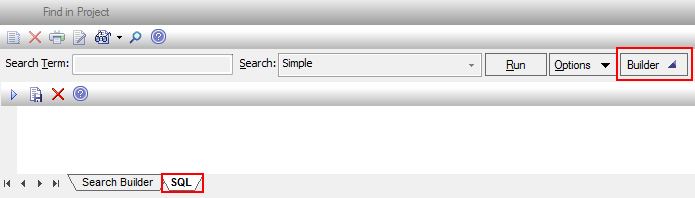
\includegraphics[width=\textwidth]{ea_activateSQLSearch}
  \caption{Advanced project search window}  
  \label{ea:builderSQLtab}
\end{center}
\end{figure}

\end{itemize}

Here you can formulate any query on the underlying database. The SQL-editor helps you with syntax-highlighting and auto-completion. Here are some basic
examples to get you started:

\begin{itemize}

\item[$\blacktriangleright$] To find all eClasses
\begin{lstlisting}[linewidth=11cm]
SELECT * FROM t_object
WHERE Object_Type='Class' AND Stereotype='eclass';
\end{lstlisting}

\item[$\blacktriangleright$] To find all associations
\begin{lstlisting}[linewidth=11cm]
SELECT * FROM t_connector
WHERE Connector_Type='Association';
\end{lstlisting}

\item[$\blacktriangleright$] To find all inheritance relations
\begin{lstlisting}[linewidth=11cm]
SELECT * FROM t_connector
WHERE Connector_Type='Generalization';
\end{lstlisting}

\item[$\blacktriangleright$] To find all connectors attaching a note to an element
\begin{lstlisting}[linewidth=11cm]
SELECT * FROM t_connector
WHERE Connector_Type='NoteLink';
\end{lstlisting}

\item[$\blacktriangleright$] To find all control flow edges (used in SDMs)
\begin{lstlisting}[linewidth=11cm]
SELECT * FROM t_connector
WHERE Connector_Type='ControlFlow';
\end{lstlisting}

\item[$\blacktriangleright$] To find all associations connected to a class named ``EClass''
\begin{lstlisting}[linewidth=11cm]
SELECT t_object.Name, t_connector.* FROM t_connector,t_object
WHERE t_connector.Connector_Type='Association'
  AND (t_connector.Start_Object_ID=t_object.Object_ID
    OR t_connector.End_Object_ID=t_object.Object_ID)
  AND t_object.Name='EClass';
\end{lstlisting}

\item[$\blacktriangleright$] To determine all subtypes of ``EClassifier''
\begin{lstlisting}[linewidth=11cm]
SELECT a.Name FROM t_connector,t_object a,t_object b
WHERE t_connector.Connector_Type='Generalization'
  AND t_connector.Start_Object_ID=a.Object_ID
  AND t_connector.End_Object_ID=b.Object_ID
  AND b.Name = 'EClassifier';
\end{lstlisting}

\item[$\blacktriangleright$] To determine all supertypes of ``EClassifier'' (cf. above)
\begin{lstlisting}[linewidth=11cm]
...
  AND t_connector.Start_Object_ID=b.Object_ID
  AND t_connector.End_Object_ID=a.Object_ID
...
\end{lstlisting}

\end{itemize}

To run the search, either hit the \texttt{Run SQL} button in the upper left corner of the editor toolbar (it shows a triangular shaped ``play'' icon), or
press \texttt{F5} on your keyboard.

\clearpage
